\documentclass{article}
\usepackage[utf8]{inputenc}

\title{TT3010 - Audio technology and room acoustics. \newline Exercise 1 - Solution Proposal}
\author{}
\date{}

\usepackage{natbib}
\usepackage{graphicx}
\usepackage{float}

\begin{document}

\maketitle


All tasks are based on chapters 10-12 in Rossings "Science of Sound" \cite{rossing}. 
It is recommended that the student will try to do every task, but tasks marked \textit{Mandatory} are to be handed in for approval (online). Deadline is November 6th.

\section*{Tasks}

\subsection*{1}

This exercise is similar to example 23.1 in Rossing book. 


Have in mind Sabines formula for reverberation (eq. 23.4 on page 532) which states:

\begin{equation}
    A = Sa
    \label{eq:abs}
\end{equation}

where A is the absorption, S is the surface area and a is the absorption coefficient.

We will also need the absorption coefficients from table 23.1 (given in the exercise).

\begin{itemize}
    \item [a.] f = 125 Hz:
    For the plastered wall, we can retrieve the absorption coefficient "plaster on lath" A using eq. \ref{eq:abs}:
    \begin{equation}
        A_{p125}=100 m^2 \cdot 0.14 = 14\ m^2
    \end{equation}
    For the carpeted concrete floor:
    \begin{equation}
        A_{c125} =100m^2 \cdot 0.02 = 2 \ m^2
    \end{equation}
    
    
    \item [b.] f = 2000 Hz : 
    \begin{equation}
        A_{p2000} = 100 m^2 \cdot 0.04 = 4\ m^2
    \end{equation}
    
    \begin{equation}
        A_{c2000}= 100 m^2 \cdot 0.6 = 60\ m^2
    \end{equation}
\end{itemize}

\begin{figure}[H]
    \centering
    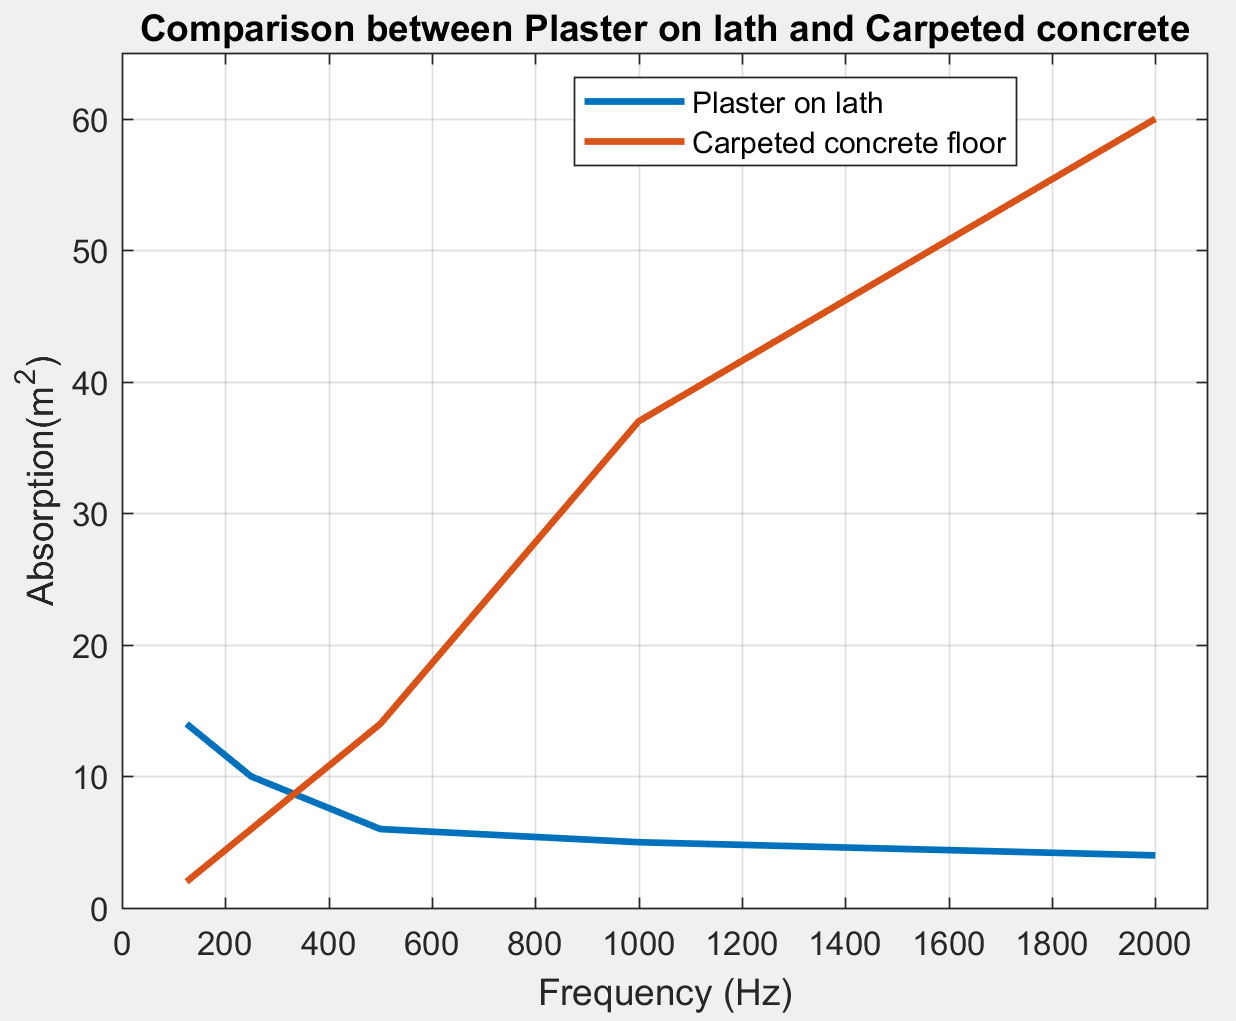
\includegraphics[scale=0.9]{figures/oving1_1.png}
    \caption{A comparison of the absorption A.}
    \label{fig:compabs}
\end{figure}

The interesting part here (as illustrated in fig. \ref{fig:compabs}), is that the plaster has higher absorption in the lower frequencies, but for higher frequencies, the carpeted concrete floor has a significantly higher absorption than the plaster. This makes sense if one has in mind that concrete reflects lower frequencies due to its massive density compared with the density of the lath. For higher frequencies, only the carpet will absorb the sound significantly. The plaster will start to vibrate at lower frequencies and absorb the sound by converting the acoustical pressure into physical energy, but for higher frequencies inherit a low absorption.

\subsection*{2}

We will use Sabine's formula and use the same approach as example 23.2 in the book. 

\begin{equation}
    RT = 0.161 \frac{V}{A}
    \label{eq:sabine}
\end{equation}

as well as coefficients from the two tables.

We will start by calculating the areas of the front-back walls, sidewalls, and floor/ceiling, and then the total absorption in the room.

\begin{equation}
    S_{fbw}=20 \cdot 15 = 300 \ m^2
\end{equation}

\begin{equation}
    S_{sw}=40 \cdot 15 = 600 \ m^2
\end{equation}

\begin{equation}
    S_{c,f}=20 \cdot 40 = 800 \ m^2
\end{equation}

\begin{equation}
    A_{f,b-wall} = 2 \cdot S_{fbw} \cdot 0.17 = 102\ m^2
\end{equation}

\begin{equation}
    A_{s-walls} = 2 \cdot S_{sw} \cdot 0.06 = 72\ m^2
\end{equation}

\begin{equation}
    A_{ceil} = S_{c,f} \cdot 0.06 = 48\ m^2
\end{equation}

\begin{equation}
    A_{floor} = S_{c,f} \cdot 0.1 = 80\ m^2
\end{equation}

\begin{equation}
    V_{auditorium} = 20 \cdot 40 \cdot 15 = 12000 \ m^3
\end{equation}

So
\begin{equation}
    A_{room} = A_{ceil}+A_{floor}+A_{s-walls}+A_{f,b-wall} = 302\ m^2
\end{equation}

\begin{itemize}
    \item [\textbf{a.}] So for empty seats:
    \begin{equation}
        A_{empty}=1100 \cdot 0.39 = 429\ m^2
    \end{equation}
    The total absorption area will be:
    
    \begin{equation}
        A_{tot} = A_{empty}+A_{room} = 731 \ m^2
    \end{equation}
    Sabines formula will then give us:
    \begin{equation}
    RT_{empty} = 0.161 \cdot \frac{V_{auditorium}}{A_{tot}}= 2.64 \ s
    \end{equation}
    
    \item [\textbf{b.}] For the case with half the seats filled, we can say that 550 seats are filled and 550 seats are empty:
    \begin{equation}
        A_{1/2-full}=550 \cdot 0.39 + 550 \cdot 0.56 = 522.5\ m^2
    \end{equation}
    The total absorption area will be:
    \begin{equation}
        A_{tot} = A_{1/2-full}+A_{room} = 824.5 \ m^2
    \end{equation}
    Sabines formula will then give us:
    \begin{equation}
    RT_{1/2-full}= 2.34 \ s
    \end{equation}
    
    \item [\textbf{c.}] When all the seats are filled, we get the following:
    \begin{equation}
        A_{full}=1100 \cdot 0.56 = 616 \ m^2
    \end{equation}
    The total absorption area will be:
    \begin{equation}
        A_{tot} = A_{full}+A_{room} = 918 \ m^2
    \end{equation}
    Sabines formula will then give us:
    \begin{equation}
    RT_{full}= 2.1 \ s
    \end{equation}
\end{itemize}

Note: Some of you have asked if there is a SI-unit that notes RT as seconds. In fact the coefficient 0.161 comes from a computation that is: $24\times ln(10)/c \approx 0.161$ s/m.

\subsection*{3}

Let's assume that a student sits exactly in the center of the room. The first sound wave from the lecturer hits the wall and ceiling at half the distance from the lecturer to the listener/student (see fig.\ref{fig:first_reflections}). 

\begin{figure}[H]
    \centering
    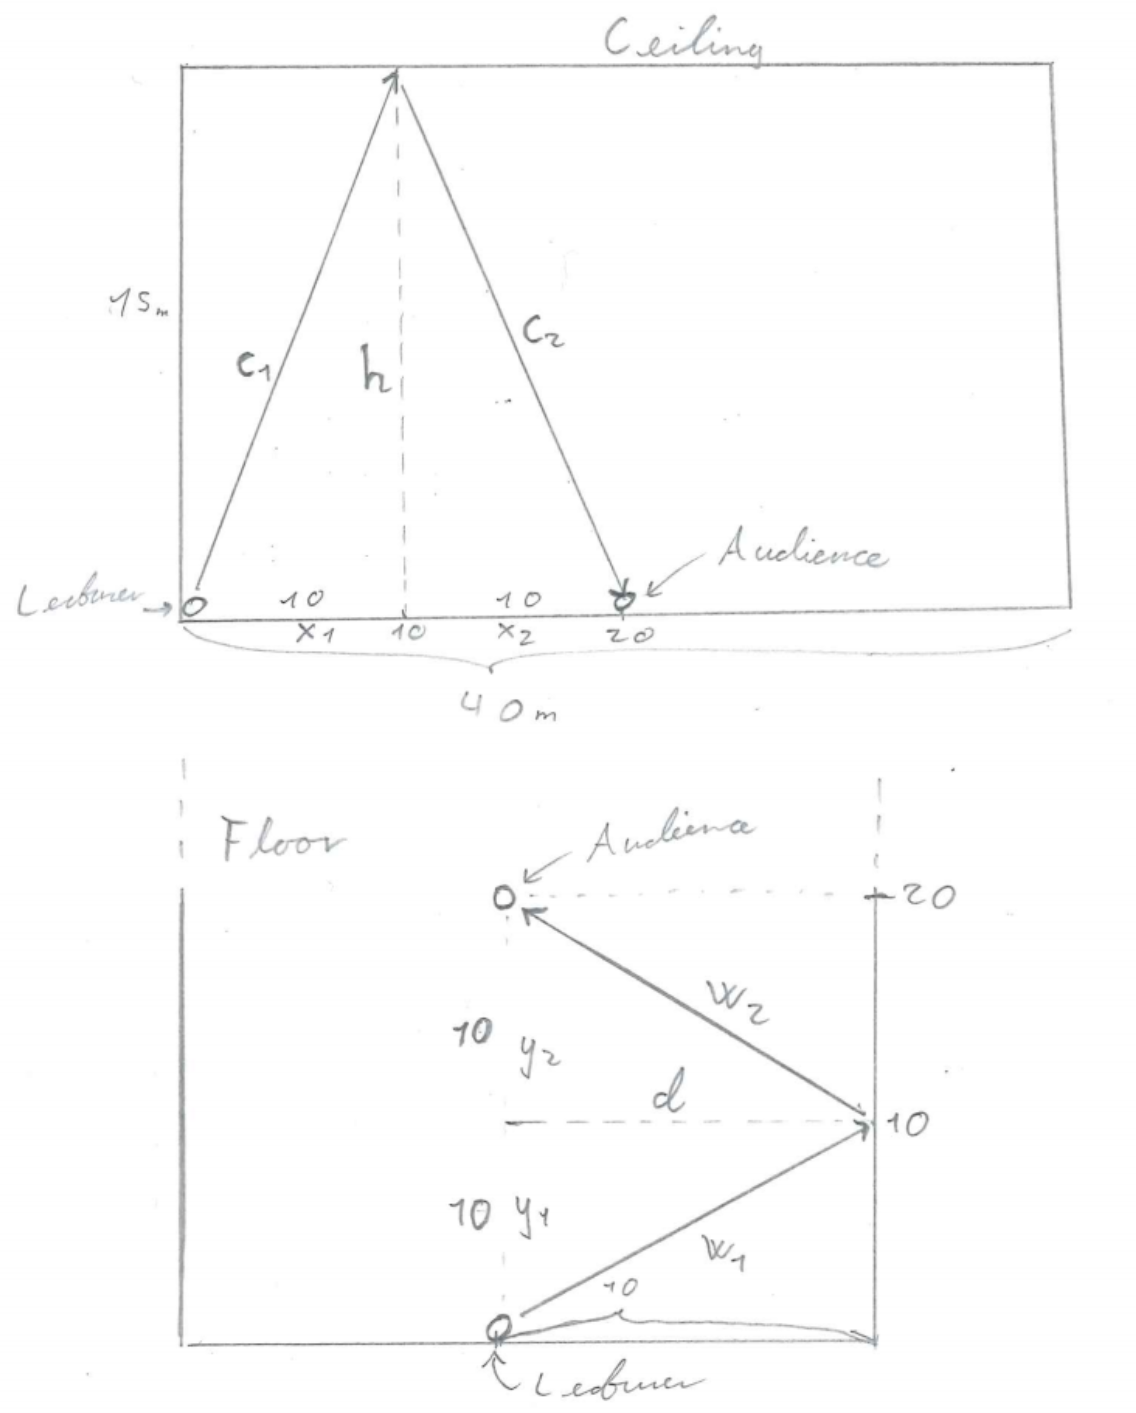
\includegraphics[scale=0.7]{figures/oving1_3.png}
    \caption{An elegant drawing of the illustrated first reflections.}
    \label{fig:first_reflections}
\end{figure}

Using Pythagoras theorem, we know that:

\begin{equation}
    L^2 = S_1^2+S_2^2
\end{equation}
where $L$ is the longest side of the triangle, and $S_1,S_2$ are the two shorter sides.
So, this gives us the following distances:

\begin{equation}
    C_1=C_2 \rightarrow C_{distance} = 2 \cdot \sqrt{x^2+h^2} \approx 36 \ m
\end{equation}

\begin{equation}
    W_1=W_2 \rightarrow W_{distance} = 2 \cdot \sqrt{y^2+d^2} \approx 28.3 \ m
\end{equation}

So, the lateral distance is shorter then the overhead distance. We can do the final step by dividing the distance with the speed of sound, $c$, and get the delays: 
\begin{equation}
  t_{1,ceil} = \frac{C_{distance}}{c} = 104\ {\rm ms}
\end{equation}

\begin{equation}
  t_{1,wall} = \frac{W_{distance}}{c} = 82\ {\rm ms}
\end{equation}

Apparently, the reflection from the sidewall, a so-called lateral reflection, arrives before the ceiling reflection. According to the book (part 23.3), it has been found that it is usually preferred that the lateral reflections arrive before the ceiling reflections since the lateral sound reflections will give a desired "spatial impression" of the room.

%although it is common knowledge that the audience in the center of a rectangular shaped auditorium receives their first reflection from the ceiling, newer studies have shown that halls with sufficiently high ceilings will have overhead reflections that are slower than the lateral reflections. 

\subsection*{4}
If the ceiling were covered with acoustical tile, our absorption ($A_{ceil}$) will have the following value:

\begin{equation}
    A_{ceil} = S_{c,f} \cdot 0.83 = 664 \ m^2
\end{equation}

The new room absorption area, $A_{room}=918\ m^2$, which means that the new reverberation times are as follow: 
\begin{equation}
RT_{empty}=0.77 s, \ \ \   
RT_{1/2-full}=0.72 s, \ \ \ 
RT_{full}= 0.67 s
\end{equation}

which is a reduction by 46 \%, 43 \% and 40 \% respectively.

\subsection*{5}

\begin{figure}[H]
    \centering
    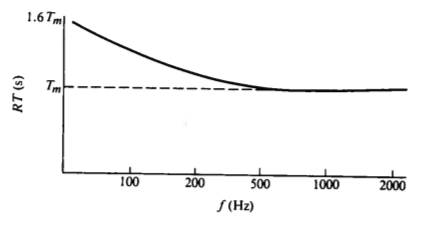
\includegraphics{figures/oving1_4.png}
    \caption{Variation of reverberation time and a good consert hall.}
    \label{fig:rt}
\end{figure}


From Rossing part 23.8 (page 535-536), we can identify the preferences of a concert hall with good acoustics. They are the following:


\begin{itemize}
    \item \textit{Intimacy or presence}. The feeling of music being played in a small hall. We can refer to 23.3 where Beranek (1996) concluded that a hall is considered intimate if the delay time between direct and first reflected sound is less than 20 ms.
    \item \textit{Reverberation, or liveness}. The persistence of a sound in a room when the tone is suddenly stopped (especially for frequencies above 350 Hz).
    \item \textit{Spaciousness, apparent width and listener envelopment}. The source appears wider than the visual width, and the sound appears to from all directions.
   \item \textit{Warmth}. The liveness of the bass tones relative to the midfrequency tones.
 
    
\end{itemize}

We see that in figure \ref{fig:rt}, the reverberation time must be higher with low frequencies. This is to get sufficient sound arriving from the sides and contribute to the feeling of spaceousness. 
Tm is a value to indicate how to 'balance' the reverberation time. For example it can be better to have a longer reverberation time at low frequency to support the bass notes and give a feeling of liveness (and this can happen because the sound absorption of a material is not the same for every frequency).

Here we can read in Figure 23.7 that the reverberation time Tm should be around 1.4s. Then looking at the Figure 23.8 we can find correcting coefficient for Tm for each frequency.


\begin{equation}
    RT_{1000} = T_{m} \cdot Coef_{1000}  = 1.4 \cdot1 =1.4\ s 
\end{equation}
\begin{equation}
    RT_{200} =  T_{m} \cdot Coef_{200} = 1.4 \cdot1.1 =1.54\ s 
    \end{equation}
    \begin{equation}
    RT_{100} = T_{m} \cdot Coef_{100} = 1.4 \cdot1.3 =1.82\ s 
\end{equation}


\subsection*{6}

According to the book(part 23.8), \textit{Flutter echoes} are a series of reflections that occur in rapid succession and are usually a result from reflections between two parallel surfaces that are highly reflective, while other surfaces are absorbing. 

Assuming a source close to one of the walls, the total distance, $D$, the sound will travel for a roundtrip is 60 m. The repetition rate, $RR$, is the number of reflections per second. In one second, the sound wave will travel a distance $L = c \cdot (1\ {\rm s}) = 343\ {\rm m}$, so the repetition rate is as follows: 

\begin{equation}
    RR = \frac{L}{D} \approx 5.7{\rm \ repetitions\ per\ second}
\end{equation}
This repetition rate corresponds to a time of 175 ms between each reflection.
Flutter-echoes behave similarly to standing waves, only with periods long enough $(>50\ ms)$ to be perceived as separate sound events. When occurring between parallel walls the axial modes normal to the parallel walls will constitute the harmonics of a flutter-echo with period T and harmonic frequencies 1/T, 2/T, etc. If the walls are hard and smooth, the higher harmonics can be prominent so that discrete tones are being heard. Due to little absorption at normal incidence and long free paths, decays are slow and reverberation time long, often leaving a late double slope at mid-high frequencies.

So, how could we illustrate this? We know that at least 5 repetitions will reach us when we have a room with a distance of 30 m between the walls. An illustration is given that shows the behaviour of the flutter echos.

\begin{figure}[H]
    \centering
    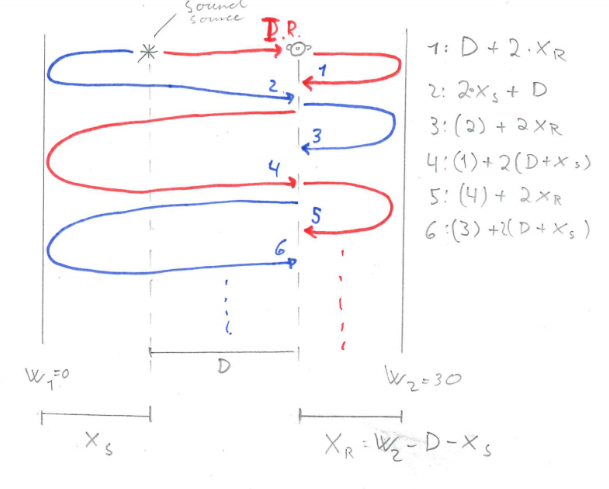
\includegraphics[scale=1.5]{figures/oving1_6.png}
    \caption{Illustrating the flutter echos traveling back and forth on the walls and hits the receiver at different times.}
    \label{fig:flutter}
\end{figure}

To reduce the effect of flutter echos, one can use curved surface deflectors to deflect as much of the direct reflections as possible.

%\subsection*{7}

%Is to be tested out. What one should find, is that for intimate room. The first reflected sound will arrive within 20 ms. 

\subsection*{7}

Assuming that the absorption in the walls is negligibly small, we are left with the following relation of Sabines equation:

\begin{equation}
    RT= 0.161 \cdot \frac{V}{mV} = \frac{0.161}{m}
\end{equation}

By using table 23.2, we can retrieve the wanted air absorption coefficient, $m$. We get:

\begin{equation}
    RT= \frac{0.161}{0.136}= 1.18 s
\end{equation}

For a room with a volume of 100 $m^3$, the result is the same!

When we think of it, it seems reasonable that if there is no absorption when the sound wave is reflected at a wall (only when the sound wave is propagating through the air) then it doesn't matter if a room is small or large - the reverberation time will be the same! We can also observe from the values for $m$ in table 23.2, that high frequencies are absorbed much more efficiently in the air than the low frequencies.

\end{document}
